% Evaluation pipeline. Build: pdflatex fig_pipeline.tex
\documentclass[tikz,border=2pt]{standalone}
\usepackage{times}
\usetikzlibrary{arrows.meta,positioning}
\begin{document}
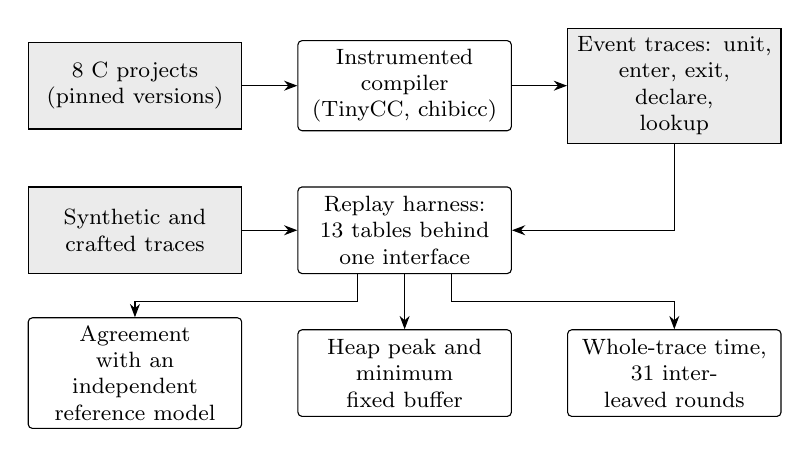
\begin{tikzpicture}[font=\footnotesize, >=Stealth, node distance=7mm and 7mm,
  blk/.style={draw, rounded corners=1.5pt, align=center, inner sep=3pt, minimum height=11mm, text width=25mm},
  dat/.style={draw, align=center, inner sep=3pt, minimum height=11mm, text width=25mm, fill=black!8}]
\node[dat] (src) {8 C projects\\(pinned versions)};
\node[blk, right=of src] (cc) {Instrumented compiler\\(TinyCC, chibicc)};
\node[dat, right=of cc] (tr) {Event traces: unit,\\enter, exit, declare,\\lookup};
\node[blk, below=of cc] (rep) {Replay harness:\\13 tables behind\\one interface};
\node[dat, left=of rep] (syn) {Synthetic and\\crafted traces};
\node[blk, below=of rep] (m2) {Heap peak and\\minimum fixed buffer};
\node[blk, left=of m2] (m3) {Agreement with an\\independent\\reference model};
\node[blk, right=of m2] (m1) {Whole-trace time,\\31 interleaved rounds};
\draw[->] (src) -- (cc);
\draw[->] (cc) -- (tr);
\draw[->] (tr.south) |- (rep.east);
\draw[->] (syn) -- (rep);
\draw[->] (rep) -- (m2);
\draw[->] (rep.south) ++(-6mm,0) -- ++(0,-3.5mm) -| (m3.north);
\draw[->] (rep.south) ++(6mm,0) -- ++(0,-3.5mm) -| (m1.north);
\end{tikzpicture}
\end{document}
